\chapter{规划}
\section{最短路径算法}
\subsection{Floyd算法}
Floyd算法采用动态规划思想,$f[k][i][j]$表示$i$和$j$之间可以通过编号为$1 \dots k$的节点的最短路径。初值$f[0][i][j]$为原图的邻接矩阵。

则$f[k][i][j]$可以从$f[k-1][i][j]$转移来,表示$i$到$j$不经过$k$这个节点。也可以从$f[k-1][i][k]+f[k-1][k][j]$转移过来,表示经过$k$这个点。意思即
\begin{equation*}
	f[k][i][j] = \rm{min}(f[k-1][i][j], f[k-1][i][k]+f[k-1][k][j])
\end{equation*}

核心代码为
\begin{lstlisting}[language=c,numbers=left,firstnumber = 1,numberstyle=\tiny,breaklines = true,keywordstyle=\color{blue!70},commentstyle=\color{red!50!green!50!blue!50},frame=shadowbox, rulesepcolor=\color{red!20!green!20!blue!20}]
	for(k=1;k<=n;k++)
        for(i=1;i<=n;i++)
            for(j=1;j<=n;j++)
                if(e[i][j]>e[i][k]+e[k][j])
                     e[i][j]=e[i][k]+e[k][j];
\end{lstlisting}

Floyd算法能够求解有向图中任意两个点之间的最短路径,且只能在不存在负权环的情况下使用,时间复杂度$O(N^3)$。

\subsection{Dijkstra算法}
Dijikstra算法采用贪心思想,维护两个点集$A$,$B$。$A$点集代表已经求出源点到该点的最短路的点的集合,$B$代表未求出源点到该点的最短路径的点的集合。维护一个向量$d$,$d[i]$代表源点到点i的最短路径长度。不断进行以下操作:找出点集$B$中$d[i]$最小的点,将这个点加入点集A中,然后用这个点到其邻接点的距离来更新向量$d$,直到点集B为空。

\href{http://wiki.jikexueyuan.com/project/easy-learn-algorithm/dijkstra.html}{\texttt{具体步骤}}为:
\begin{enumerate}
\item 将所有的顶点分为两部分:已知最短路程的顶点集合 P 和未知最短路径的顶点集合 Q。最开始,已知最短路径的顶点集合 P 中只有源点一个顶点。我们这里用一个 book[ i ]数组来记录哪些点在集合 P 中。例如对于某个顶点 i,如果 book[ i ]为 1 则表示这个顶点在集合 P 中,如果 book[ i ]为 0 则表示这个顶点在集合 Q 中。
\item 设置源点 s 到自己的最短路径为 0 即 dis=0。若存在源点有能直接到达的顶点 i,则把 dis[ i ]设为 e[s][ i ]。同时把所有其它(源点不能直接到达的)顶点的最短路径为设为 ∞。
\item 在集合 Q 的所有顶点中选择一个离源点 s 最近的顶点 u(即 dis[u]最小)加入到集合 P。并考察所有以点 u 为起点的边,对每一条边进行松弛操作。例如存在一条从 u 到 v 的边,那么可以通过将边 u->v 添加到尾部来拓展一条从 s 到 v 的路径,这条路径的长度是 dis[u]+e[u][v]。如果这个值比目前已知的 dis[v]的值要小,我们可以用新值来替代当前 dis[v]中的值。
\item 重复第 3 步,如果集合 Q 为空,算法结束。最终 dis 数组中的值就是源点到所有顶点的最短路径。
\end{enumerate}

Dijkstra算法能够求解图中单源点到其他所有点的最短路径。时间复杂度为$O(N^2)$

\subsection{Bellman-Ford算法}
\href{http://www.cnblogs.com/gaochundong/p/bellman_ford_algorithm.html}{\texttt{具体步骤}}为:
\begin{enumerate}
	\item 创建源顶点 v 到图中所有顶点的距离的集合 distSet,为图中的所有顶点指定一个距离值,初始均为 Infinite,源顶点距离为 0;
	\item 计算最短路径,执行V-1次遍历: 对于图中的每条边, 如果起点 u 的距离 d 加上边的权值 w 小于终点 v 的距离 d,则更新终点 v 的距离值 d;
	\item 检测图中是否有负权边形成了环: 遍历图中的所有边,计算 u 至 v 的距离,如果对于 v 存在更小的距离,则说明存在环;
\end{enumerate}

Bellman-Ford算法也能解决单源最短路问题,且对边的情况没有要求,不仅可以处理负权边,还能处理负环。时间复杂度为$O(V\times E)$

\subsection{A*算法}
个人理解A*算法只是针对搜索方向的一种启发式处理方法,在寻找最短路径的搜索过程中,通常都是以Dijkstra算法为基础进行的。具体的伪代码为:
\begin{lstlisting}[language=c,numbers=left,firstnumber = 1,numberstyle=\tiny,breaklines = true,keywordstyle=\color{blue!70},commentstyle=\color{red!50!green!50!blue!50},frame=shadowbox, rulesepcolor=\color{red!20!green!20!blue!20}]
function A*(start, goal)
    // The set of nodes already evaluated
    closedSet := {}

    // The set of currently discovered nodes that are not evaluated yet.
    // Initially, only the start node is known.
    openSet := {start}

    // For each node, which node it can most efficiently be reached from.
    // If a node can be reached from many nodes, cameFrom will eventually contain the
    // most efficient previous step.
    cameFrom := an empty map

    // For each node, the cost of getting from the start node to that node.
    gScore := map with default value of Infinity

    // The cost of going from start to start is zero.
    gScore[start] := 0

    // For each node, the total cost of getting from the start node to the goal
    // by passing by that node. That value is partly known, partly heuristic.
    fScore := map with default value of Infinity

    // For the first node, that value is completely heuristic.
    fScore[start] := heuristic_cost_estimate(start, goal)

    while openSet is not empty
        current := the node in openSet having the lowest fScore[] value
        if current = goal
            return reconstruct_path(cameFrom, current)

        openSet.Remove(current)
        closedSet.Add(current)

        for each neighbor of current
            if neighbor in closedSet
                continue		// Ignore the neighbor which is already evaluated.

            if neighbor not in openSet	// Discover a new node
                openSet.Add(neighbor)
            
            // The distance from start to a neighbor
            //the "dist_between" function may vary as per the solution requirements.
            tentative_gScore := gScore[current] + dist_between(current, neighbor)
            if tentative_gScore >= gScore[neighbor]
                continue		// This is not a better path.

            // This path is the best until now. Record it!
            cameFrom[neighbor] := current
            gScore[neighbor] := tentative_gScore
            fScore[neighbor] := gScore[neighbor] + heuristic_cost_estimate(neighbor, goal) 

    return failure

function reconstruct_path(cameFrom, current)
    total_path := [current]
    while current in cameFrom.Keys:
        current := cameFrom[current]
        total_path.append(current)
    return total_path
\end{lstlisting}
上述伪代码可以用于移动机器人路径搜索。其中closedSet表示已经搜索过的位置,openSet表示待搜索的位置。从openSet中按照fScore的值找到最近的待搜索点,从openSet中移入closedSet中。更新该点相邻可达点的fScore值和cameFrom表,同时将相邻点(不在closedSet)加入openSet中。不断重复直到搜索到达目标点,然后根据cameFrom表逆推得到最短路径。

与Dijkstra算法相比,A*算法最核心的地方就是对距离函数的取值:
\begin{equation*}
	f(n) = g(n) + h(n)
\end{equation*}
其中,$g(n)$就是Dijkstra算法中计算出的从源点到当前点的距离,$h(n)$则表示当前点到目标点的距离估计。利用该估计值启发搜索方向。这是我用Matlab编写的\href{/attachment/myastar.m}{\texttt{A*代码}}。为了便于Matlab搜索和定位,代码中将二维坐标转换为了一维坐标处理。

\section{路径搜索算法}
\subsection{PRM算法}
概率路图(Probabilistic RoadMap, PRM)算法。基本步骤分为两步:先对地图进行预处理建图,生成可行路径无向图,然后查询源点、终点在图上对应的最短距离。

\noindent {\hei $\blacksquare$ PRM算法预处理步骤}

\begin{enumerate}
\item 地图随机采样,生成中间路径点。
\item 按照不同的方法,在路径点之间生成路径
\item 对路径进行碰撞检测。
\end{enumerate}

在PRM算法中,常规方式是逐点采样,然后按照半径距离$r$连接到已生成的图中;一种简化方法(sPRM)是一次生成N个采样点,然后再逐点生成路径。此外,对最近若干点的挑选方式也有不同处理。常规是按照给定的半径球内寻点。k-Nearest (s)PRM 始终搜寻最近的k个点生成路径。Bounded-degree (s)PRM 则是对常规方式的球内点添加了k个最近上限。


\subsection{RRT算法}
快速扩展随机树(Rapidly-exploring Random Trees, RRT)算法。本节主要参考\href{http://rkala.in/codes/RRT.zip}{\texttt{Rahul Kala}}的代码以及\href{http://www.cnblogs.com/21207-iHome/p/7210543.html}{\texttt{这篇博客}}。

\noindent {\hei $\blacksquare$ RRT算法步骤}

\begin{enumerate}
\item 初始化随机树,确定初始点、目标点,地图尺寸、地图障碍物位置等
\item 随机采样。按照一定的概率在地图中挑选随机点或是用目标点作为当前采样点$q_\rm{rand}$
\item 选取最近节点。在当前随机树中找出与采样点最近的节点,作为扩展节点$q_\rm{nearest}$
\item 随机树扩展。沿$q_\rm{nearest}$和$q_\rm{rand}$方向,按照一定步长生成新节点$q_\rm{new}$
\item 碰撞检测。若$\overrightarrow{q_\rm{nearest} q_\rm{new}}$上的点都与障碍物无碰撞,则将$q_\rm{new}$加入随机树中。
\item 若$q_\rm{new}$距离目标点足够近则停止搜索,否则跳转步骤2。
\end{enumerate}

在实际使用是,还需要考虑:如何进行随机采样?如何定义“最近”以及如何快速搜索到最近节点(Kd-Tree)?如何进行扩展等。博客中举了一个车型机器人的例子,显然车的前后移动要比旋转、航向移动要方便,对应与更“近”。

\noindent {\hei $\blacksquare$ Bidirectional RRT/RRT Connect}

单源点开始搜索的RRT算法在搜索效率上仍显的较慢,因此有人提出如下的双向RRT搜索算法。
\begin{figure}[htbp]
	\figskip 
	\centering
	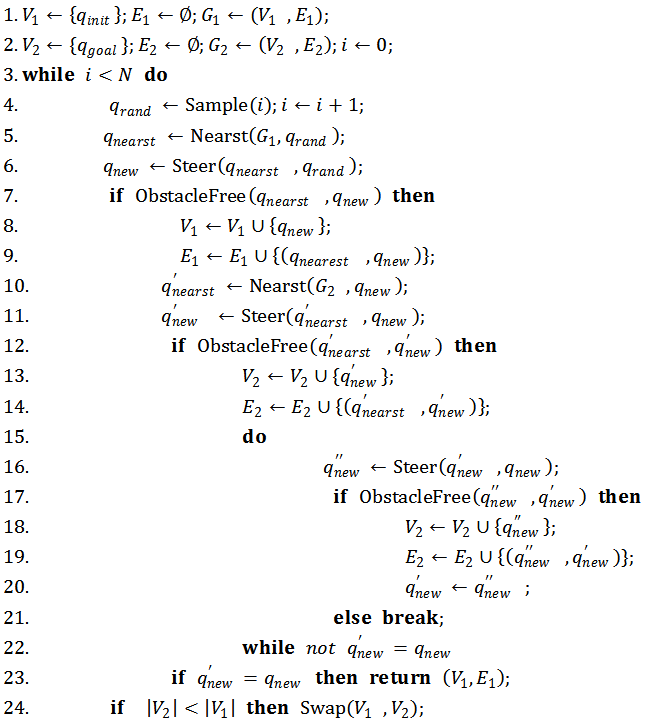
\includegraphics[width = 0.85\textwidth,trim = 0 -0 0 -0,clip]{rrt-connect.png}	  
	\caption{\label{fig: rrt-connect} RRT-Connect算法步骤}
\end{figure}
基本思想可以理解为:先对源点做一次RRT搜索,然后用扩展点对终点做一次RRT搜索,然后用源点RRT的扩展点与终点RRT的扩展点再做连续RRT拓展,直到遇到障碍物。然后重复上述步骤。为了平衡两棵随机树的节点,每一步搜索中的第一次的RRT可以对节点数多的进行。

\subsection{RRT*算法}
最优RRT(RRT*)算法,主要参考\href{/attachment/Sampling-based Algorithms for Optimal Motion Planning10.1.1.419.5503.pdf}{\texttt{这篇论文}}。简单来说,RRT*算法的“最优”性体现在对随机树的动态优化上,基本思想为:

\begin{enumerate}
    \item 随机树扩展。对于待扩展的新节点$q_\rm{new}$,不是简单的生成从$q_\rm{nearest}$到$q_\rm{new}$的路径,而是在$q_\rm{new}$的一个邻域内搜索所有节点$q_\rm{near}$,使得源点经过$q_\rm{near}$到$q_\rm{new}$的路径最短,这时再添加$q_\rm{near}$到$q_\rm{new}$路径。
    \item 随机树修正。对$q_\rm{new}$邻域内所有节点$q_\rm{near}$再做一次搜索,若源点经过新节点$q_\rm{new}$到$q_\rm{near}$的距离更短,则变更$q_\rm{near}$的父节点为$q_\rm{new}$,且替换原路径。
\end{enumerate}

\begin{figure}[htbp]
	\figskip 
	\centering
	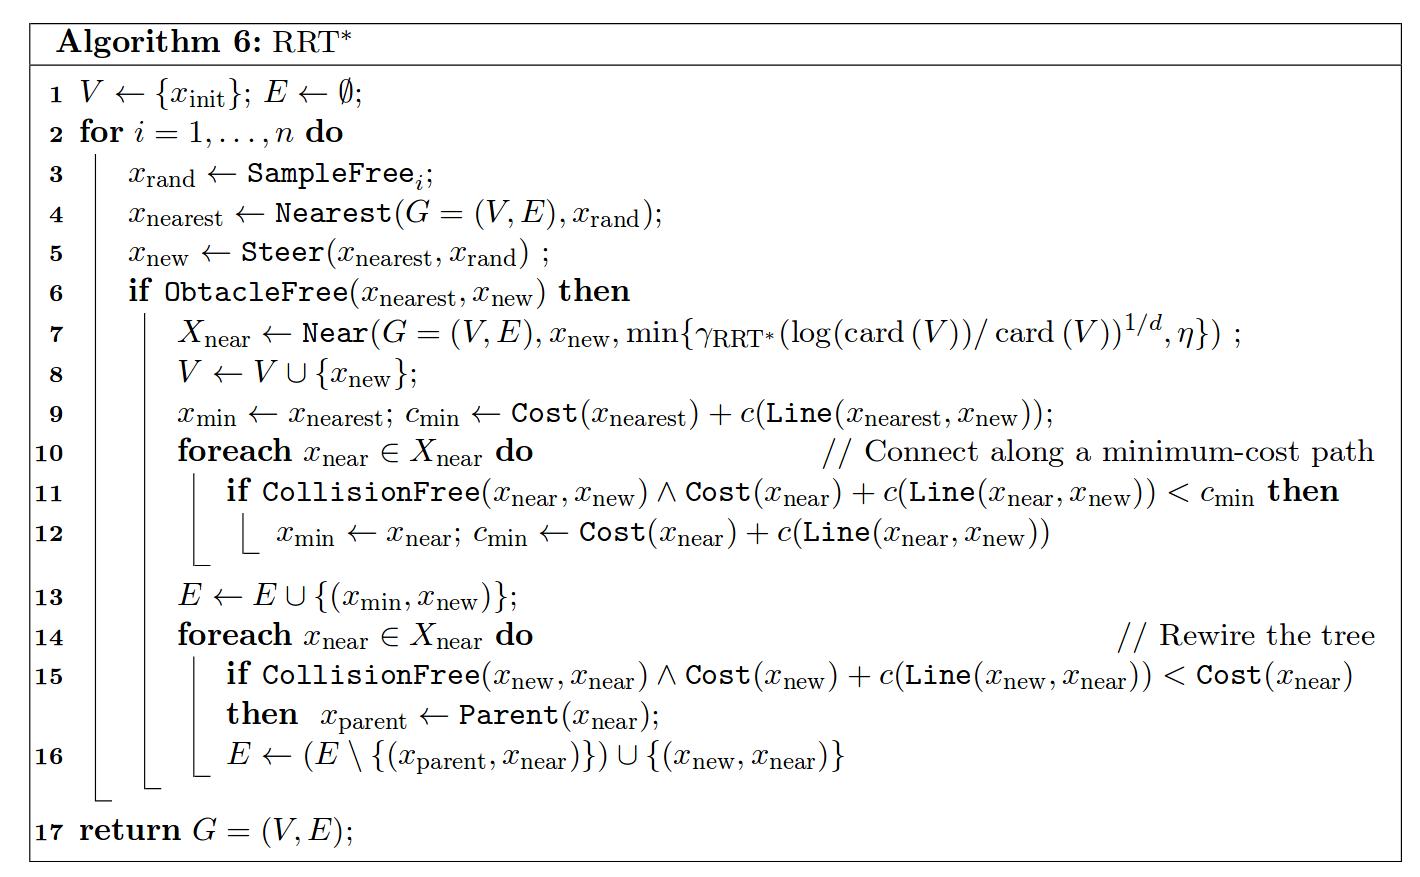
\includegraphics[width = 0.9\textwidth,trim = 0 -0 0 -0,clip]{RRT*.png}	  
	\caption{\label{fig: RRT*} RRT*算法伪代码}
\end{figure}

\noindent {\hei $\blacksquare$ 疑问}

RRT*算法在每一步搜索中都需要寻找$q_\rm{new}$的邻域节点,这个搜索的代价是不是太大?如果按照常规RRT算法生成节点和路径,最后再做一次全局的最短路径搜索,性能对比如何?

\section{路径曲线生成算法}
\subsection{Dubins path}
对于平面路径生成,可以用$(x,y,\psi)'$表示状态,其中$x,y$为轨迹点的平面坐标位置,$\psi$表示轨迹点运动的轨迹偏角(对无人机,假设无侧滑角飞行)。Dubins曲线采用圆弧和直线连接源点和终点,对于包含直线的Dubins曲线,按照源点转弯方向和终点转弯方向,可以分为RSR,RSL,LSR,LSL共四种曲线形式。

\begin{figure}[htbp]
	\figskip 
	\centering
	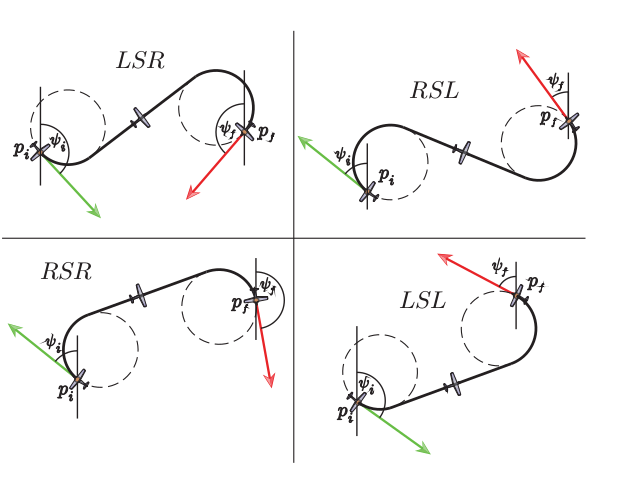
\includegraphics[width = 0.75\textwidth,trim = 0 -0 0 -0,clip]{Dubins.png}	  
	\caption{\label{fig: Dubins} 四种Dubins曲线形式}
\end{figure}

具体算法思想可以参考\href{/attachment/Dubins.pdf}{\texttt{这篇论文}},具体的MATLAB实现可以看
\href{/attachment/dubins.m}{\texttt{这里}},主要注意下坐标系(x轴指向北)与论文中不一样,实现过程比较简单,都是几何运算。

基本思路都是:
\begin{enumerate}
	\item 按照路径形式确定源点、终点的转弯圆心
	\item 按照路径形式确定两圆的切线方向、航迹偏角
	\item 计算圆上切点
	\item 计算转弯旋转角度的变化增量
\end{enumerate}

关于如何根据条件状态直接选择路程最短的形式,可以参考王师姐论文。

\subsection{Bezier曲线 和 B-spline曲线}
\noindent {\hei $\blacksquare$ 贝塞尔曲线}

参考\href{https://www.cnblogs.com/hnfxs/p/3148483.html}{\texttt{这篇博客}}。给定源点$P_0$和终点$P_1$,那么一阶Bezier曲线就是这两个点的连线,连线上的点可以描述为:
\begin{equation*}
    P = (1-t)P_0 + tP_1
\end{equation*}
其中,$t: 0 \Rightarrow 1$。这个形式相当于一个一阶插值。类似的,二阶Bezier曲线中,一共需要3个控制点$P_0$,$P_1$,$P_2$,先计算$P_0$和$P_1$的曲线点$P_0^1$,再计算$P_1$和$P_2$的曲线点$P_1^1$,最后计算$P_0^1$和$P_1^1$的曲线点就是二阶曲线上的点。

\begin{align*}
    P &= (1-t)\left[(1-t)P_0 + tP_1\right] + t\left[ (1-t)P_1 + tP_2\right] \\
      &= (1-t)^2 P_0 + 2t(1-t)P_1 + t^2 tP_2
\end{align*}

贝塞尔曲线存在的问题:
\begin{enumerate}
	\item 确定了多边形的顶点数(m个),也就决定了所定义的Bezier曲线的阶次(m-1次),不够灵活。
    \item 当顶点数(m)较大时,曲线的阶次将比较高。此时,多边形对曲线形状的控制将明显减弱。    
    \item Bezier的调和函数的值,在开区间(0,1)内均不为0。因此,所定义的曲线在(0<t<1)的区间内的任何一点均要受到全部顶点的影响,即改变其中任一个顶点的位置,都将对整条曲线产生影响,因此对曲线进行局部修改是不可能的。
\end{enumerate}

\noindent {\hei $\blacksquare$ B样条曲线}

可以参考\href{https://blog.csdn.net/Mr_Grit/article/details/45603627}{\texttt{这篇博客}}。讲的比较清楚,而且代码也可以运行通过。

一般使用其中的准均匀B样条曲线,需要特别注意其中求取节点的地方,包括数量及其分布。节点可以理解为在原控制点上的扩充,用于计算基函数。控制点就是给定的控制多边形的定点。




\subsection{其他形式曲线}
\noindent {\hei $\blacksquare$ Reeds-Shepp曲线}

与Dubins曲线相比,RS曲线中机器人既能够前向运动,也能够后向运动(类似具有倒车的性质)。共计9类46种曲线直线组合结果。

\noindent {\hei $\blacksquare$ Balkcom-Mason曲线}

与RS曲线相比,Balkcom-Mason曲线中机器人可以绕中心旋转(类似双轮机器人差动转向的性质)。

\noindent {\hei $\blacksquare$ Pythagorean Hodograph曲线}

PH曲线是一种具有有理特性的参数化多项式曲线。具体计算可以根据师姐论文中的方法,在复平面内进行计算。

\subsection{多项式轨迹}
通过路径搜索算法可以找到一系列的离散路径点,通过多项式曲线将这些点连接起来形成多项式轨迹。本节的主要算法参考\href{https://pdfs.semanticscholar.org/2376/078d13761387cabb933798b93a706c2ea7ef.pdf}{\texttt{论文A}}
和\href{http://www-personal.acfr.usyd.edu.au/spns/cdm/papers/Mellinger.pdf}{\texttt{论文B}}。其中对于多项式轨迹的基本内容可以阅读教材 Trajectory Planning for Automatic Machines and Robots Springer 第二章中的相关部分。

对于本节的多项式轨迹生成问题,可以转化为求解一个二次规划(QP, Quadratic Program)问题。
假设多项式的系数可以表示为$\bm{p} = [p_0, p_1, \cdots, p_n]^T$,多项式函数为$P(t)$ 那么采用论文A中的目标函数:

\begin{equation}
    J(T) = \int_0^T c_0 P(t)^2 + c_1 P'(t)^2 + c_2 P''(t)^2 + \cdots + c_N P^{(N)}(t)^2 \dd t = \bm{p}^T Q(T) \bm{p}
\end{equation}
其中,$Q(T)$ 为Hessian矩阵,可以通过简单的微积分运算求解。$T$表示每一段多项式轨迹的总时间。
对于M+1个离散路径点,共需要生成M段多项式轨迹,这样总的目标函数可以表示为:

\begin{equation}
J_{total} = \begin{bmatrix} \bm{p}_1 \\ \vdots \\ \bm{p}_M \end{bmatrix}^T 
 \begin{bmatrix} Q_1(T_1) & & \\ & \ddots & \\ & & Q_M(T_M) \end{bmatrix}
 \begin{bmatrix} \bm{p}_1 \\ \vdots \\ \bm{p}_M \end{bmatrix}^T 
\end{equation}

对于二次规划问题可以通过现成的工具箱进行求解,所以剩下的问题就是如何将轨迹生成中的边界约束转化为二次规划的约束形式。
{\color{red}此外需要注意的是上述目标函数中需要指定每一段的轨迹时间,这些时间量可以作为上一层优化问题的优化变量。}

从无人机飞行动力学考虑,一种合理的假设是飞行过程中无人机位置、速度、加速度是连续变化的,每一段的边界条件也是位置、速度、加速度这三个变量。
那么对于任意一段多项式轨迹,初始边界条件3个,终端边界条件3个,因此需要最少5次多项式(6个系数)才能满足所有边界条件。对每一段多项式的边界条件可以描述为:
\begin{equation}
    \bm{A}_i \bm{p}_i = \bm{d}_i
\end{equation}
对于5次多项式,考虑P、V、A三项边界时,上述三项展开为:
\begin{equation}
    \bm{A}_i = \begin{bmatrix}
        1   & t_0   & t_0^2     & t_0^3     & t_0^4     & t_0^5 \\
        0   & 1     & 2 t_0     & 3 t_0^2   & 4 t_0^3   & 5 t_0^4 \\
        0   & 0     & 2         & 6 t_0     & 12 t_0^2  & 20 t_0^3 \\
        1   & t_T   & t_T^2     & t_T^3     & t_T^4     & t_T^5 \\
        0   & 1     & 2 t_T     & 3 t_T^2   & 4 t_T^3   & 5 t_T^4 \\
        0   & 0     & 2         & 6 t_T     & 12 t_T^2  & 20 t_T^3 
    \end{bmatrix}
\end{equation}

\begin{equation}
    \bm{d}_i = [P_0, \, V_0, \, A_0, \, P_T, \, V_T, \, A_T]^T
\end{equation}

在实际规划过程中,常常并不知道无人机到达中间离散路径点位置时的速度、加速度,因此需要使用连续边界条件,即
\begin{equation}
    A_{T,i} \bm{p}_i = A_{0,i+1} \bm{p}_{i+1}
\end{equation}




